\documentclass[12pt, letterpaper]{article}
\usepackage[utf8]{inputenc}
\usepackage{graphicx}
\usepackage{float}
\usepackage{amsmath}
\usepackage{tikz}
\usepackage{pgfplots}


\begin{document}
	
	% Title page
	\begin{titlepage}
		\begin{center}
			\line(1,0){340}\\
			[0.25in]
			\huge\bfseries Fitting a Curve to Points via Ordinary Least Squares
			\line(1,0){340}\\
			[1.1cm]
			\textsc{\Large by: Jabari Dash}\\
		\end{center}
	\end{titlepage}

%---------------------------------------------------------------------

	\tableofcontents
	
%---------------------------------------------------------------------

	\newpage
	
	\section{What Is Curve Fitting?} 
		\subsection{What is it?}
			\paragraph{}
				Suppose we are given a set of data points that take the form $(x, y)$. The points appear to have a \textit{trend} to them - such as a linear or parabolic relationship. But, at the moment, the only thing that we know about them is their coordinates. \textbf{Curve fitting} is the process of analyzing these data points, performing some operations on them, and extracting an \textit{equation} or \textit{curve} that explains the relationship of the points in our data set.	
				
				\begin{figure}[H]
					\begin{center}
						% Graph the newly found equation crossing the points
						\begin{tikzpicture}
						% Draw x and y axis from -2 to 5 inclusive, with respective labels
						\draw (-2,0) -- coordinate (x axis mid) (5,0) node[right] {$x$};
						\draw (0,-2) -- coordinate (y axis mid) (0,5) node[above] {$y$};	
						
						% Draw ticks and label x-axis
						\foreach \x in {-2,...,5}
						\draw (\x,1pt) -- (\x,-3pt) node[anchor=north] {\x};
						
						% Draw ticks and label y-axis
						\foreach \y in {-2,...,5}
						\draw (1pt,\y) -- (-3pt,\y) node[anchor=east] {\y}; 
						
						% Draw point at (2,3)
						\coordinate (A) at (2,3);
						\draw (A) circle[radius = 4pt];
						\node at (A) [above = 3mm] {$(2,3)$};
						\fill (A) circle[radius = 4pt];
						
						% Draw point at (3,4)
						\coordinate (B) at (3,4);
						\draw (B) circle[radius = 4pt];
						\node at (B) [above = 3mm] {$(3,4)$};
						\fill (B) circle[radius = 4pt];
						\end{tikzpicture}
					\end{center}
					\caption{Two arbitrary points}
				\end{figure}
				
			\paragraph{}
				There are several ways to fit a curve to points. For example, in a high school algebra class we are given questions such as "Given points $(2,3)$ and $(3,4)$, find a line that passes through each point." Naturally, we do the following:
				
				\begin{equation}
					y=mx+b
				\end{equation}
				
				\begin{equation}
					m=\frac{\Delta{y}}{\Delta{x}}=\frac{y_2-y_1}{x_2-x_1}
				\end{equation}
				
				\begin{equation}
					m=\frac{3-2}{4-3}=\frac{1}{1}=1
				\end{equation}
				
				\begin{equation}
					b=y-mx
				\end{equation}
				
				\begin{equation}
					b=3-(1\cdot{2})
				\end{equation}
				
				\begin{equation}
					b=3-2=1
				\end{equation}
				
				\begin{equation}
					\boxed{y=x+1}
				\end{equation}
				
				\begin{figure}[H]
					% put in center, because \boxed forces left align
					
					\begin{center}
						% Graph the newly found equation crossing the points
						\begin{tikzpicture}
							% Draw x and y axis from -2 to 5 inclusive, with respective labels
							\draw (-2,0) -- coordinate (x axis mid) (5,0) node[right] {$x$};
							\draw (0,-2) -- coordinate (y axis mid) (0,5) node[above] {$y$};	
							
							% Draw ticks and label x-axis
							\foreach \x in {-2,...,5}
							\draw (\x,1pt) -- (\x,-3pt) node[anchor=north] {\x};
							
							% Draw ticks and label y-axis
							\foreach \y in {-2,...,5}
							\draw (1pt,\y) -- (-3pt,\y) node[anchor=east] {\y}; 
								
							% Draw line of equations y = x + 1				
							\draw[thick, <->] [scale=1,domain=-3:4,smooth,variable=\x, red] plot ({\x},{\x+1}) node [right = 3mm] {$y=x+1$};
							
							% Draw point at (2,3)
							\coordinate (A) at (2,3);
							\draw (A) circle[radius = 4pt];
							\node at (A) [above = 3mm] {$(2,3)$};
							\fill (A) circle[radius = 4pt];
							
							% Draw point at (3,4)
							\coordinate (B) at (3,4);
							\draw (B) circle[radius = 4pt];
							\node at (B) [above = 3mm] {$(3,4)$};
							\fill (B) circle[radius = 4pt];
						\end{tikzpicture}
					\end{center}
					\caption{Linear fit to the 2 points}
				\end{figure}
			
		\subsection{Why do it?}			
			\paragraph{}
				The high school approach is a perfectly valid approach. However, it has some limitations and makes some assumptions. For example, if we were asked to find a a line that intersects the points $(2,3)$, $(3,4)$, and $(5,3)$, we would not be able to solve this problem. That is because the line does not exist. We would be search forever via the high school method because it \textit{assumes} that the line exists. If the line does exist, there is a perfect match for the points, and the equation that we get back. 
		
		\begin{figure}[H]	
				% put in center, because \boxed forces left align
				\begin{center}
					% Graph the newly found equation crossing the points
					\begin{tikzpicture}
					% Draw x and y axis from -2 to 5 inclusive, with respective labels
					\draw (-2,0) -- coordinate (x axis mid) (5,0) node[right] {$x$};
					\draw (0,-2) -- coordinate (y axis mid) (0,5) node[above] {$y$};	
					
					% Draw ticks and label x-axis
					\foreach \x in {-2,...,5}
					\draw (\x,1pt) -- (\x,-3pt) node[anchor=north] {\x};
					
					% Draw ticks and label y-axis
					\foreach \y in {-2,...,5}
					\draw (1pt,\y) -- (-3pt,\y) node[anchor=east] {\y}; 
					
					% Draw line of equations y = x + 1				
					\draw[thick, <->] [scale=1,domain=-3:4,smooth,variable=\x, red] plot ({\x},{\x+1}) node [right = 3mm] {$y=x+1$};
					
					% Draw point at (2,3)
					\coordinate (A) at (2,3);
					\draw (A) circle[radius = 4pt];
					\node at (A) [above = 3mm] {$(2,3)$};
					\fill (A) circle[radius = 4pt];
					
					% Draw point at (3,4)
					\coordinate (B) at (3,4);
					\draw (B) circle[radius = 4pt];
					\node at (B) [above = 3mm] {$(3,4)$};
					\fill (B) circle[radius = 4pt];
					
					% Draw point at (1,1)
					\coordinate (C) at (1,1);
					\draw (C) circle[radius = 4pt];
					\node at (C) [right = 3mm] {$(1,1)$};
					\fill (C) circle[radius = 4pt];
					\end{tikzpicture}
				\end{center}
				\caption{The 3rd point is not intersected by our line}
			\end{figure}
				
			\paragraph{}
				But what do we do when we do not have a \textit{perfect} match? We can try connecting the different pairs, and \textit{see} which line \textit{looks} like that best fit? 
			
			\begin{figure}[H]	
				% put in center, because \boxed forces left align
				\begin{center}
					% Graph the newly found equation crossing the points
					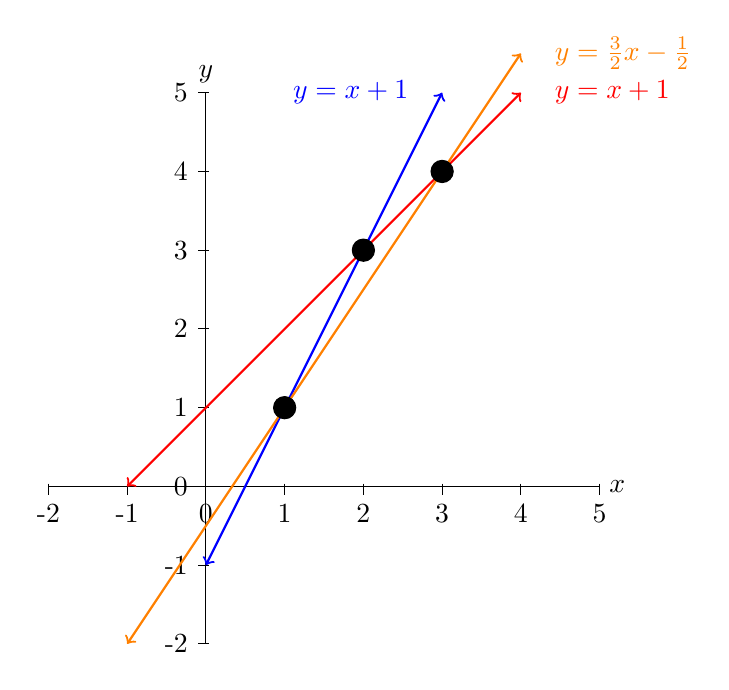
\begin{tikzpicture}
					% Draw x and y axis from -2 to 5 inclusive, with respective labels
					\draw (-2,0) -- coordinate (x axis mid) (5,0) node[right] {$x$};
					\draw (0,-2) -- coordinate (y axis mid) (0,5) node[above] {$y$};	
					
					% Draw ticks and label x-axis
					\foreach \x in {-2,...,5}
					\draw (\x,1pt) -- (\x,-3pt) node[anchor=north] {\x};
					
					% Draw ticks and label y-axis
					\foreach \y in {-2,...,5}
					\draw (1pt,\y) -- (-3pt,\y) node[anchor=east] {\y}; 
					
					% Draw line of equations y = x + 1				
					\draw[thick, <->] [scale=1,domain=0:3,smooth,variable=\x, blue] plot ({\x},{(2 *\x)-1}) node [left = 3mm] {$y=x+1$};
					
					% Draw line of equations y = x + 1				
					\draw[thick, <->] [scale=1,domain=-1:4,smooth,variable=\x, red] plot ({\x},{\x+1}) node [right = 3mm] {$y=x+1$};
					
					% Draw line of equations y = x + 1				
					\draw[thick, <->] [scale=1,domain=-1:4,smooth,variable=\x, orange] plot ({\x},{(3 / 2 * \x) -.5}) node [right = 3mm] {$y=\frac{3}{2}x-\frac{1}{2}$};
					
					% Draw point at (2,3)
					\coordinate (A) at (2,3);
					\draw (A) circle[radius = 4pt];
					\fill (A) circle[radius = 4pt];
					
					% Draw point at (3,4)
					\coordinate (B) at (3,4);
					\draw (B) circle[radius = 4pt];
					\fill (B) circle[radius = 4pt];
					
					% Draw point at (1,1)
					\coordinate (C) at (1,1);
					\draw (C) circle[radius = 4pt];
					\fill (C) circle[radius = 4pt];
					\end{tikzpicture}
				\end{center}
				\caption{We find lines via the high school method}
			\end{figure}
				
			\paragraph{}	
				We see here that the high school method is already getting out of hand because we have 3 potential best fit lines, and we only have 3 points. If we were given a data set of ten, or one-hundred data points, it would be impossible (or would take a really long time) to find all of the lines, and choose the best one. Not to mention, that we also have not designed a method of measuring which one is the \textit{best fit}. This is the reason why mathematicians have designed more \textit{general} curve fitting solutions. It turns out the the \textit{best fit} equation is $y=\frac{3}{2}x-\frac{1}{3}$ and was computed via the \textbf{Least Squares} method.
			
			\begin{figure}[H]	
				% put in center, because \boxed forces left align
				\begin{center}
					% Graph the newly found equation crossing the points
					\begin{tikzpicture}
					% Draw x and y axis from -2 to 5 inclusive, with respective labels
					\draw (-2,0) -- coordinate (x axis mid) (5,0) node[right] {$x$};
					\draw (0,-2) -- coordinate (y axis mid) (0,5) node[above] {$y$};	
					
					% Draw ticks and label x-axis
					\foreach \x in {-2,...,5}
					\draw (\x,1pt) -- (\x,-3pt) node[anchor=north] {\x};
					
					% Draw ticks and label y-axis
					\foreach \y in {-2,...,5}
					\draw (1pt,\y) -- (-3pt,\y) node[anchor=east] {\y}; 
					
					% Draw line of equations y = 1.5x - 1/3				
					\draw[thick, <->] [scale=1,domain=-1:3.5,smooth,variable=\x, red] plot ({\x},{(1.5 *\x) - (1/3)}) node [left = 3mm] {$y=\frac{3}{2}x-\frac{1}{3}$};
					
					% Draw point at (2,3)
					\coordinate (A) at (2,3);
					\draw (A) circle[radius = 4pt];
					\fill (A) circle[radius = 4pt];
					
					% Draw point at (3,4)
					\coordinate (B) at (3,4);
					\draw (B) circle[radius = 4pt];
					\fill (B) circle[radius = 4pt];
					
					% Draw point at (1,1)
					\coordinate (C) at (1,1);
					\draw (C) circle[radius = 4pt];
					\fill (C) circle[radius = 4pt];
					\end{tikzpicture}
				\end{center}
				\caption{We use Least Squares to find a best fit line}
			\end{figure}
			
	
	\section{What is Least Squares?}
		\subsection{Linear Regression}

		\subsection{Non-linear Regression}
	
	\section{Linear Fit} 
		
	\section{Polynomial Fit}
	
	\section{Exponential Fit}
	
	\section{Logarithmic Fit}
	
	\section{Sinusoidal Fit}
	
	\section{References}
	
	
\end{document}